%!TEX root = ./../projectReport.tex

\chapter{Usability} % (fold)
\label{cha:usability}
To perform the commands shown in this chapter, please navigate to the C++-project folder ('turbulence').


\section{Project folder} % (fold)
\label{sec:project_folder}

NS-EOF can still be run by writing into the shell the following command:

\bashh{SCENARIOS/run.txt}{1}

\noii However, we advice to run the Python-script 'run' both on the cluster and locally to start the simulation\footnote{For more informations on the options, we refer to the help:
\bashh{SCENARIOS/runh.txt}{1}
}:

\bashh{SCENARIOS/runl.txt}{1}

\noii By doing so, the simulation is started but also a new folder is created containing all relevant files of the simulation. This folder is referenced in the following as project folder.

\noii By copying and placing all the input files (configuration file, backup file for initialisation, geometry file) and all the result files (output, VTK files, backup file, timing results) into one folder the user is enabled to completely understand the simulation at a later time.

\noii The following tree shows the structure of the project folder:
\dirtree{%
.1 project.
.2 job.cmd.
.2 log.
.2 out.
.2 petsc\_commandline\_arg.
.2 scenario.xml.
.2 timing/.
.3 ....
.2 vtks/.
.3 ....
}

\noii The next sections describe two input files (the configuration and the geometry files) in more detail.

\clearpage

\section{Configuration file} % (fold)
\label{sec:configuration_file}

For the sake of completeness, a configuration file is shown in its original appearance as provided at the beginning of the lab course. 

\noii It contains the setup for a DNS simulation of a backward facing step scenario with a streched mesh.

\xmll{SCENARIOS/conf-reference.xml}{2}

\noii All additional new options are shown in the following sections in reference to this file.

\noii \textbf{Tested configuration files} can be found in the 'scenarios'-folder.

\newpage
\subsubsection*{Algebraic turbulence model}

For the second worksheet, the group implemented an algebraic turbulence model with different methods to limit the mixing length and thus the eddy viscosity (nulimiter=1: no limitation; =3 limitation with the help of a laminar flat plate Blasius boundary layer; =4 limitation with the help of a turbulent flat boundary layer). 

\xmll{SCENARIOS/type-aturb.xml}{2}

\noii A laminar simulation with this implementation can be performed by setting $\nu_t$ to zero (type='laminar'). The results should be comparable with the DNS-simulation (\citep{lienen2015} p.~14).  

\subsubsection*{k-$\varepsilon$ turbulence model}

The user can use alternatively to the algebraic turbulence model the k-$\varepsilon$ model to calculate the eddy viscosity. Following optional parameters can be set:
\begin{itemize}
\item model constants $C_{\varepsilon 1}$, $C_{\varepsilon 2}$, $\sigma_k$, $\sigma_\varepsilon$ and $C_{\mu}$ (see equation~\ref{equ:constants})
\item wall near treatment (model=0: no wall modifications, =1: Lam and Bremhorst, =2: Chien, =3: Jones and Launder, =4 Fan and Lakshminarayana)
\item adaptive time stepping (number of refinements and permitted error)
\item solving quasi laminarily for the first 'start' seconds (not solving the transport equations for $k$ and $\varepsilon$ and setting $\nu_T=0$)
\end{itemize}

\xmll{SCENARIOS/type-ke.xml}{2}

\noii A laminar simulation with this implementation can be performed by setting $\nu_t$ to zero (type='laminar').

\subsubsection*{Scenarios}

As described in section~\ref{sec:new_scenarios}, additional scenarios were added:

\begin{itemize}
\item symmetrical channel
\xmll{SCENARIOS/scenario-channel-symm.xml}{1}
\item boundary layer over a flat plate
\xmll{SCENARIOS/scenario-boundary.xml}{1}
\item free shear flow (without any side walls)
\xmll{SCENARIOS/scenario-free.xml}{1}
\end{itemize}

\subsubsection*{Inlet}

For every scenario except for 'cavity', the velocity inlet profile in x-direction can be prescribed as either uniform (true) or parabolic (false).

\xmll{SCENARIOS/scenario-uniform.xml}{1}

\subsubsection*{Flow around arbitrary geometry}

The user can specify a reference to a geometry file (see: \ref{sec:geometry_file}) to be used to set up an obstacle in any scenario.

\xmll{SCENARIOS/ageom.xml}{2}



\subsubsection*{Backup files}

The user can specify the backup (.bak) files to be used for initialisation and for saving the results of the final time step. Backup files are written after every interval specified by the user and at the end of the simulation.

\xmll{SCENARIOS/restart.xml}{2}

\noii No file ending '.bak' needs to be specified in the configure file.

% subsection configuration_file (end)

\clearpage

\section{Geometry file} % (fold)
\label{sec:geometry_file}

The geometry file (.geo) contains the coordinates of all obstacle cells. Each line represents exactly one obstacle cell and has the following format (with the first number i, the second number j and the third number k):

\xmll{SCENARIOS/geo.txt}{2}

\noii The team developed two Matlab-scripts for creating files of the necessary format for 2D geometries:
\begin{itemize}
\item \underline{Scripting}:\\
The user specifies with a basic function which position is in the geometry and which is in the flow field. The Matlab-script evaluates this function for the middle point of each cell and writes the file. Elementary geometries (circle, square, plate) and geometries composed by these forms can be created:

\begin{figure}[!htb]
\centering
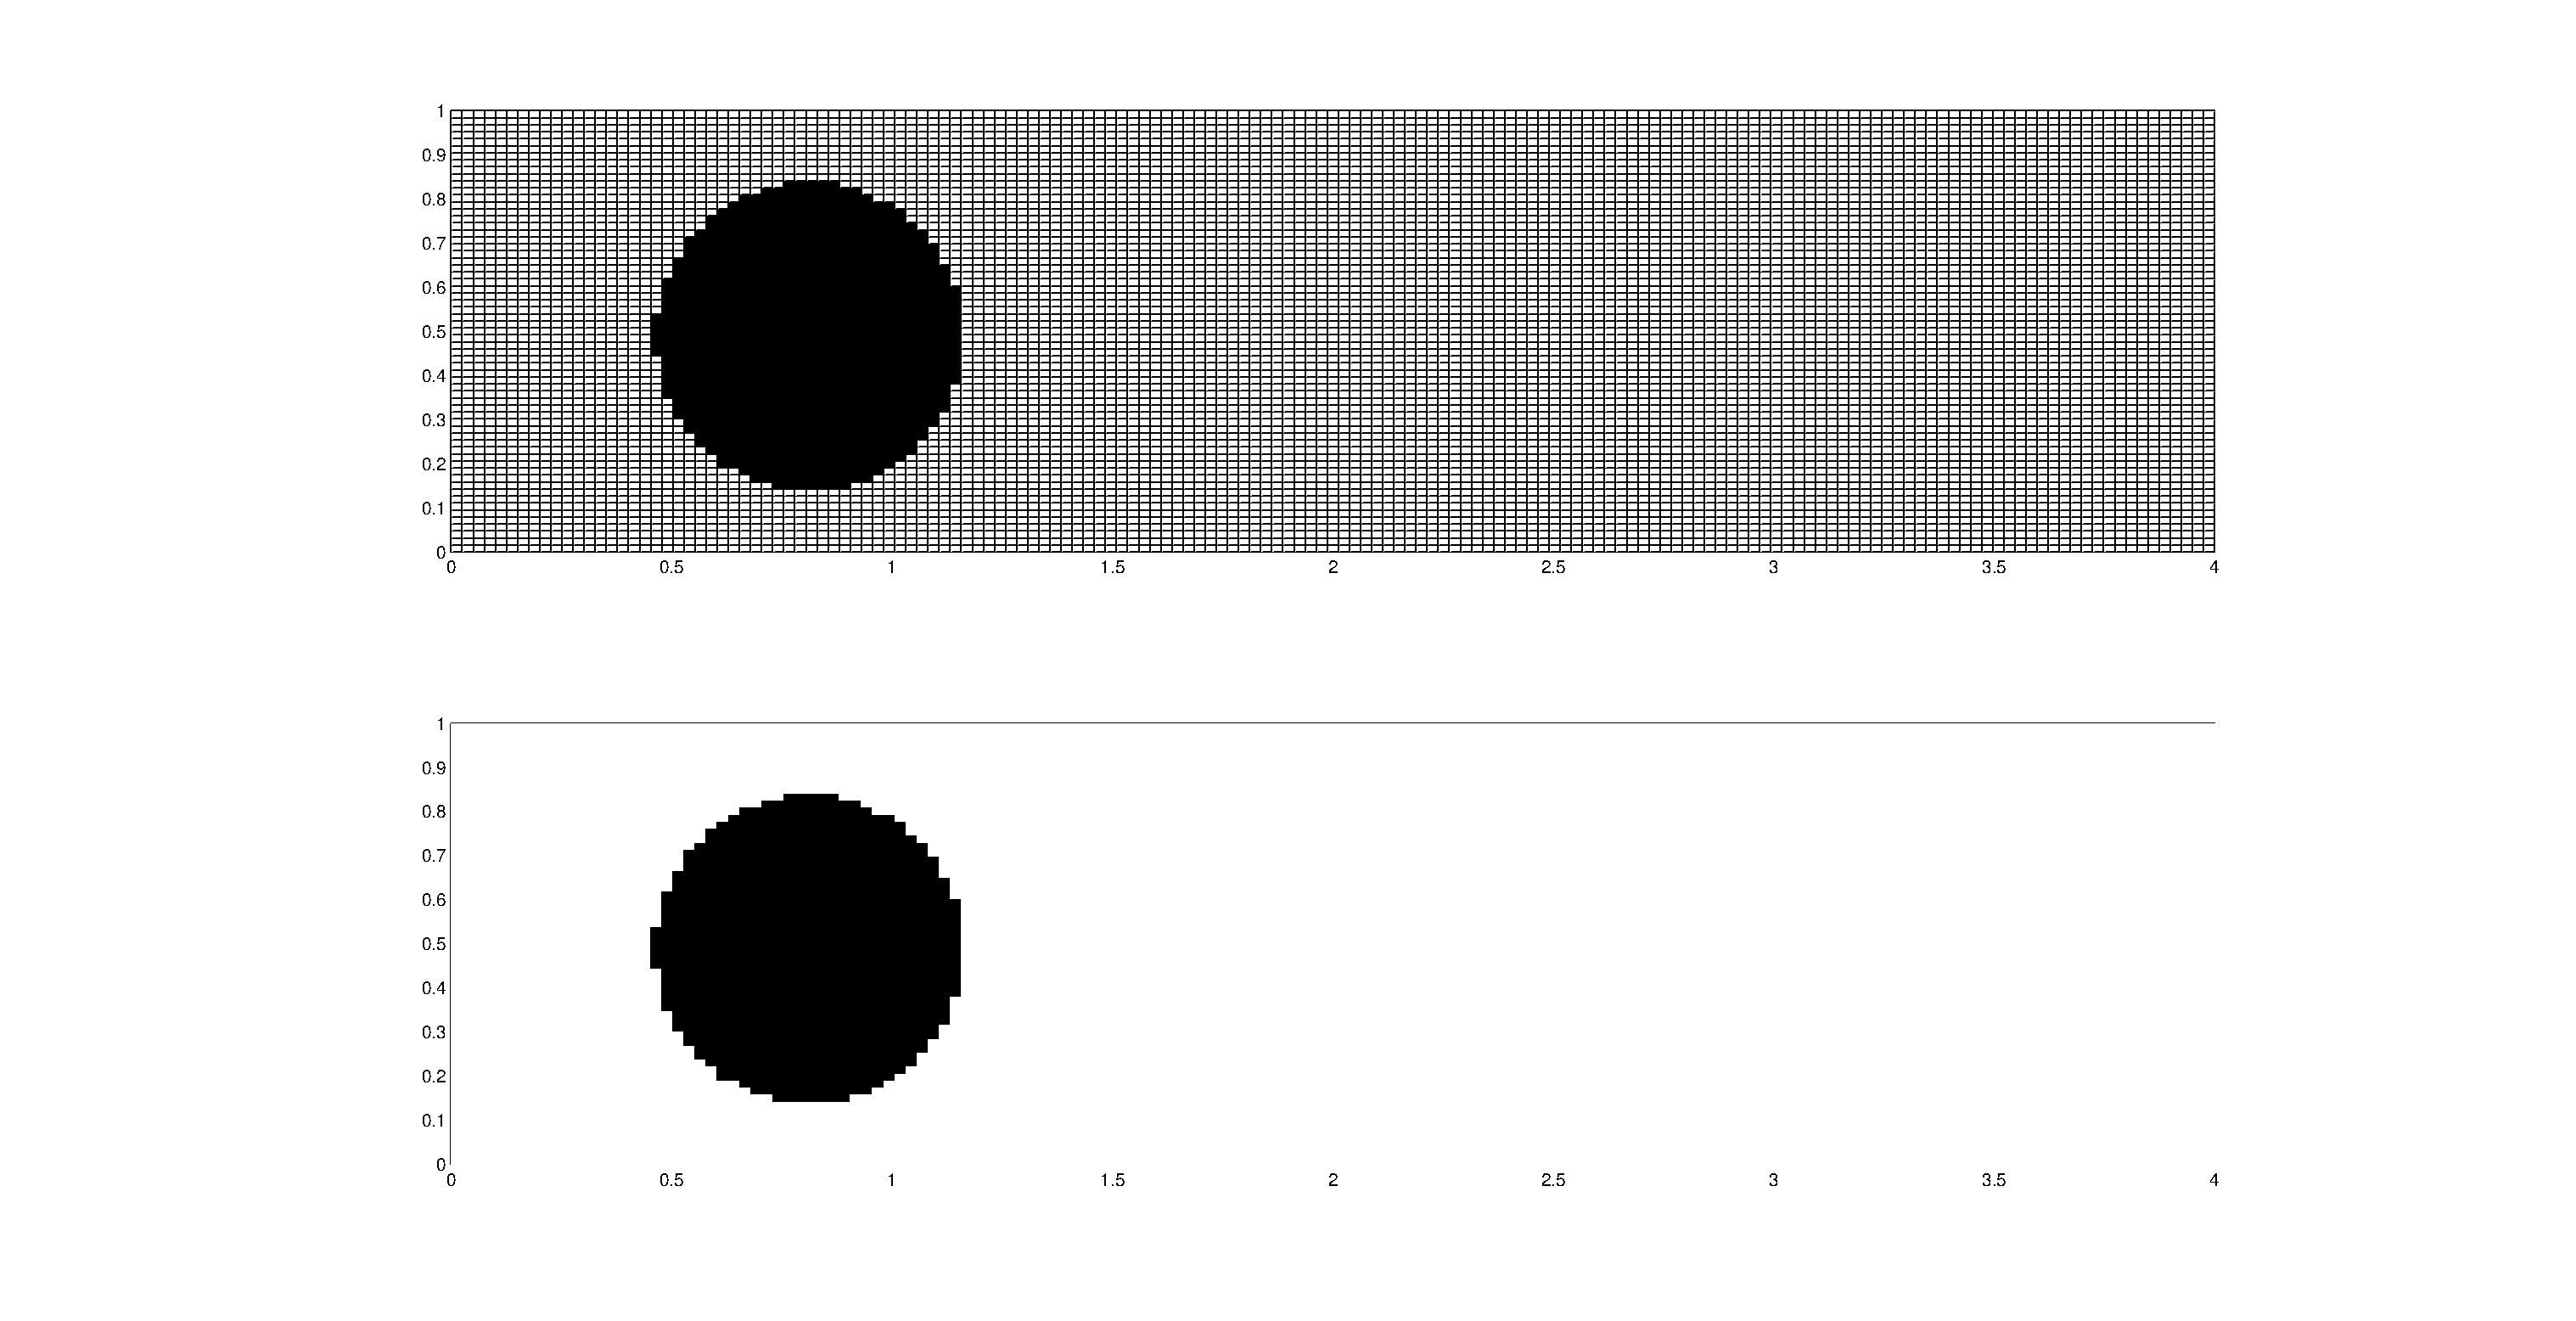
\includegraphics[scale=.3]{FIGURES/circle.eps}
\caption{Circle in a channel}
\label{fig:circle_in_channel}
\end{figure} 

\item \underline{Drag \& Drop}:\\
The second possibility to create arbitrary geometries is given by an interactive matlab script. The runnable script can be found in the script folder ns-eof-geogui and is called turbulence.m.
When running the script, a coordinate system with limits set according to the specified number of points in x- and y-direction shows up first. Based on this coordinate system, the surrounding line of an obstacle can be chosen.

Therefore, the starting point of the surrounding line has to be specified by a mouse click by the user\footnote{ It is recommended to keep starting point in mind.}
After that, the following points defining the surrounding line have to be chosen in the right consecutive order (lines between the already chosen points will show up in the coordinate frame).

To close the geometry, the point which was chosen as starting point has to be clicked again. Afterwards, the edges of the geometry can be seen in the coordinate frame.

In a next step, a point somewhere in the middle of the specified obstacle has to be clicked on. It will be used as starting point for a recursive algorithm to detect all cells lying inside the obstacle.

After this point is selected, all necessary user inputs are given and the geometry file is written in a text file.

In the figure below, an example (the created profile of an airfoil) is shown.


\begin{figure}[!htb]
\centering
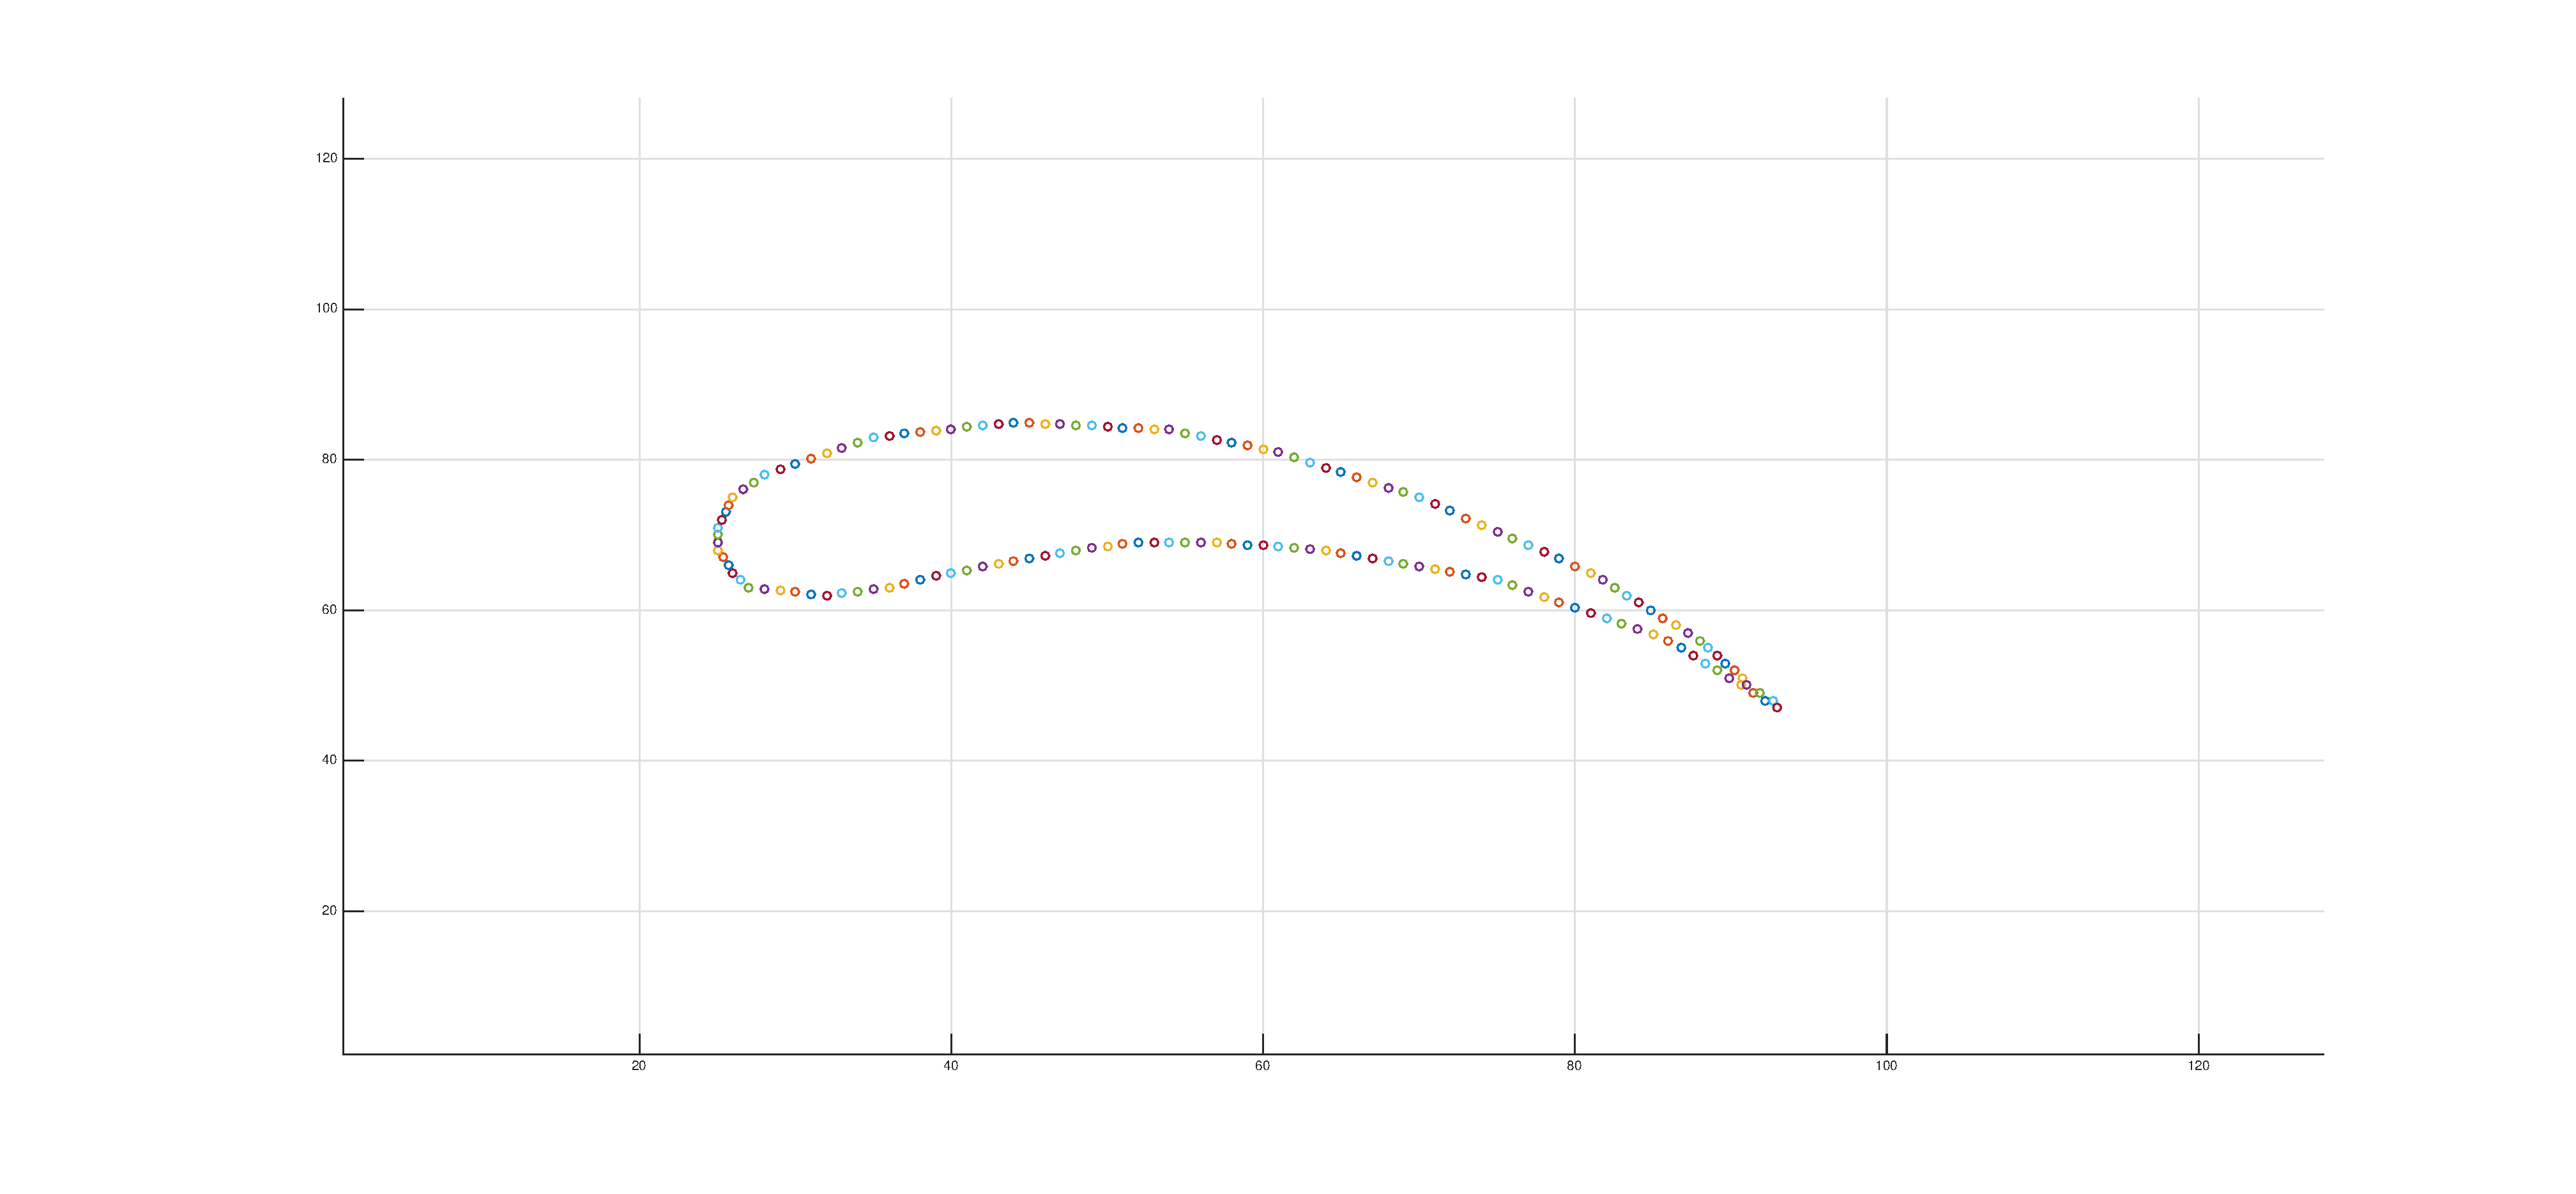
\includegraphics[scale=.23]{FIGURES/airfoil.eps}
\caption{Airfoil in a channel}
\label{fig:circle_in_channel}
\end{figure} 

\end{itemize}



% subsection geometry_file (end)

% chapter usability (end)